\documentclass{ximera}

\title{What is a limit?}

\newenvironment{objectives}{\begin{remark}\textbf{Objectives}\\}{\end{remark}}

\begin{document}
\begin{abstract}
\end{abstract}

\subsection{Quiz}

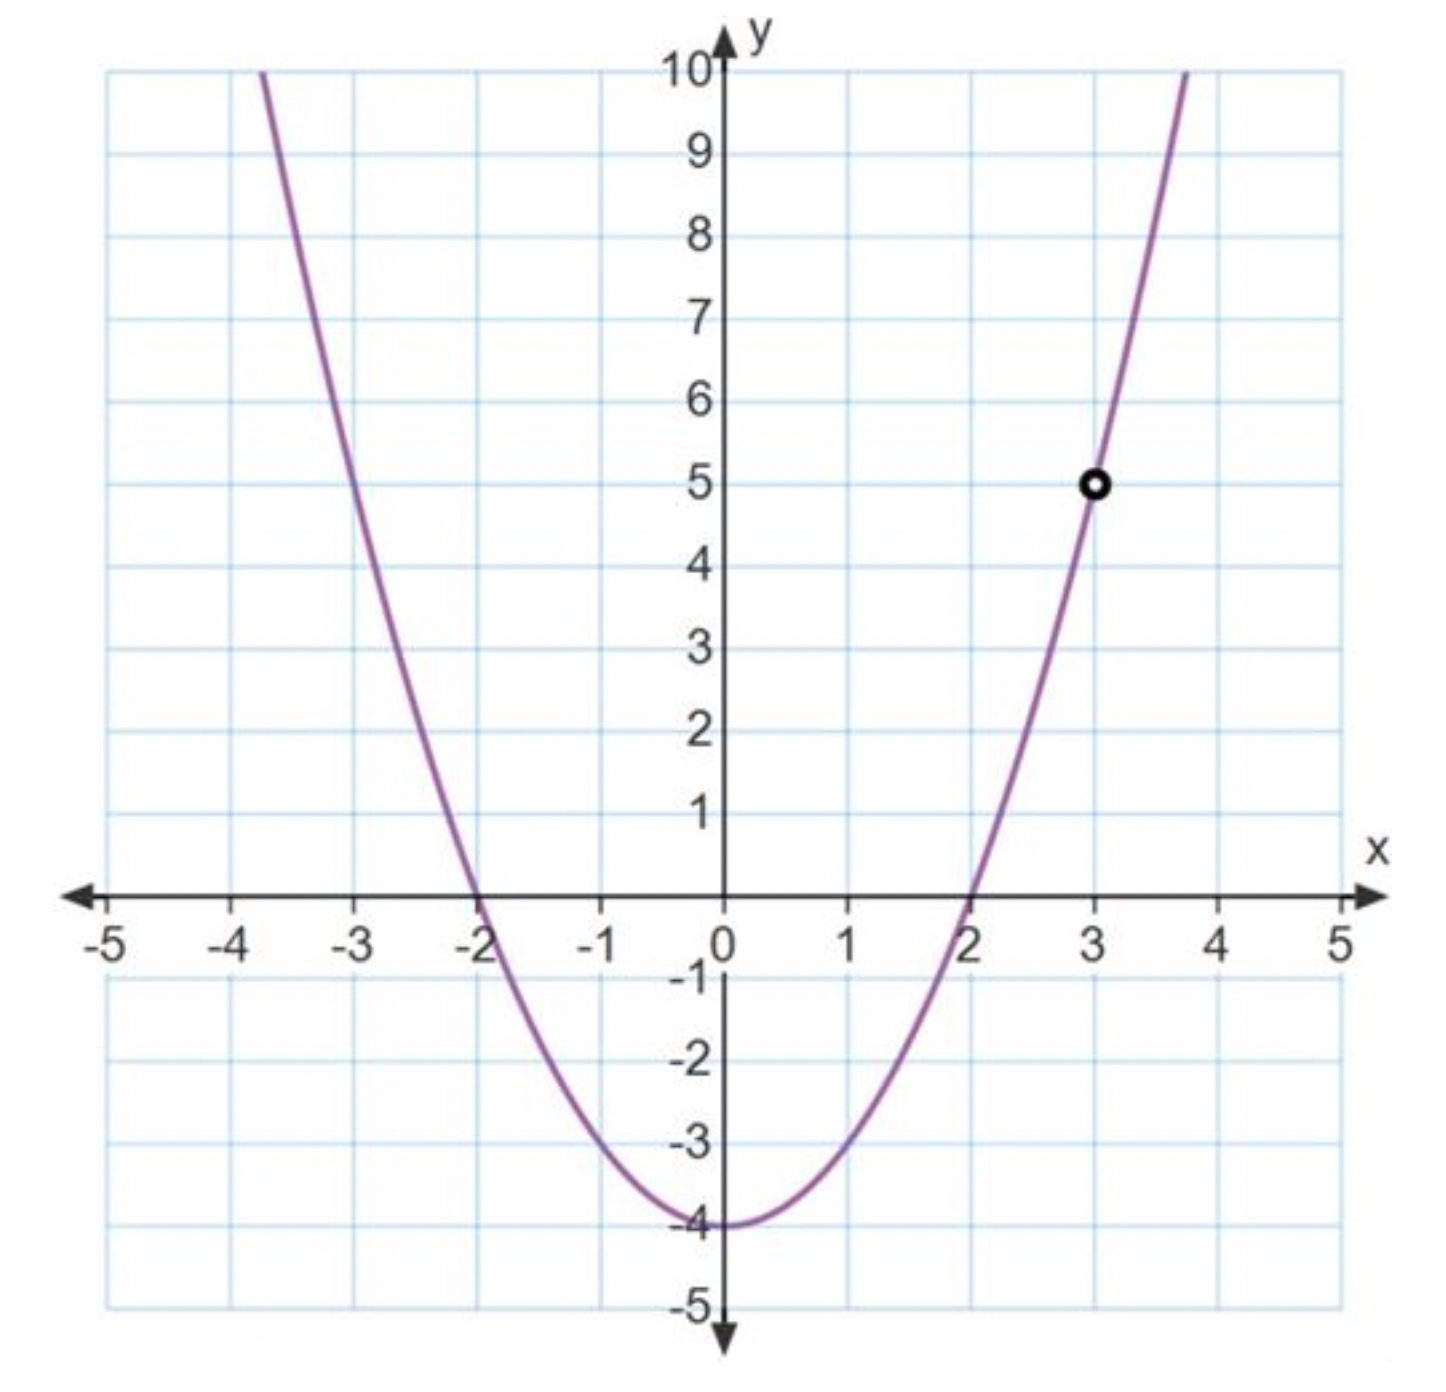
\includegraphics[width=0.5\textwidth]{graph1.png}
\begin{question}  
$\lim_{x \to 3} f(x) = \answer{5}$  

% \begin{exploration}
\begin{explanation}
    That's right! You selected the correct response. The limit as $x$ approached $3$ is $5$. This is the $y$-value the graph is getting close to when the $x$-value is near $3$.
% \end{exploration}
\end{explanation}
\end{question}


\end{document}